\documentclass[tikz, twoside, fleqn]{article}
\usepackage{graphicx, fancyhdr, amsmath, amssymb, amsthm, subfig, url, hyperref}
\usepackage[backend=biber, style=alphabetic]{biblatex}
\usepackage[margin=1in]{geometry}
\usepackage[brazilian]{babel}
\usepackage[utf8]{inputenc}
\usepackage{mathtools}
\usepackage{float}
\usepackage{lastpage}
\usepackage{listings}
\usepackage{pgfplots}
\usepackage{xcolor}
\usepackage{nameref}
\usepackage{csquotes}

\addbibresource{bibliography.bib}
%----------------------- Macros and Definitions --------------------------
% Cores definidas pelo usuario
\definecolor{mygreen}{RGB}{28,172,0}
\definecolor{mylilas}{RGB}{170,55,241}

% Imagens e eixos
\pgfplotsset{compat=1.10}
\usetikzlibrary{pgfplots.fillbetween, backgrounds}

% Configuração de orientacao do Tikz
\tikzset{
    reverseclip/.style={insert path={(current page.north east) --
        (current page.south east) --
        (current page.south west) --
        (current page.north west) --
        (current page.north east)}
    }
}

% Listar secoess
\setcounter{secnumdepth}{0}

% Configuracoes do matlab
\lstset{language=Matlab,%
    breaklines=true,%
    morekeywords={matlab2tikz},
    keywordstyle=\color{blue},%
    morekeywords=[2]{1}, keywordstyle=[2]{\color{black}},
    identifierstyle=\color{black},%
    stringstyle=\color{mylilas},
    commentstyle=\color{mygreen},%
    showstringspaces=false,
    numbers=left,%
    numberstyle={\tiny \color{black}},
    numbersep=9pt,
    emph=[1]{for,end,break},emphstyle=[1]\color{red}, %some words to emphasise
    %emph=[2]{word1,word2}, emphstyle=[2]{style},    
}

% Equações 
\makeatletter
\newcommand*\@dblLabelI {}
\newcommand*\@dblLabelII {}
\newcommand*\@dblequationAux {}

\def\@dblequationAux #1,#2,%
    {\def\@dblLabelI{\label{#1}}\def\@dblLabelII{\label{#2}}}

\newcommand*{\doubleequation}[3][]{%
    \par\vskip\abovedisplayskip\noindent
    \if\relax\detokenize{#1}\relax
       \let\@dblLabelI\@empty
       \let\@dblLabelII\@empty
    \else % we assume here that the optional argument
          % has the required shape A,B
       \@dblequationAux #1,%
    \fi
    \makebox[0.5\linewidth-1.5em]{%
     \hspace{\stretch2}%
     \makebox[0pt]{$\displaystyle #2$}%
     \hspace{\stretch1}%
    }%
    \makebox[0.5\linewidth-1.5em]{%
     \hspace{\stretch1}%
     \makebox[0pt]{$\displaystyle #3$}%
     \hspace{\stretch2}%
    }%
    \makebox[3em][r]{(%
  \refstepcounter{equation}\theequation\@dblLabelI, 
  \refstepcounter{equation}\theequation\@dblLabelII)}%
  \par\vskip\belowdisplayskip
}
\makeatother

\renewcommand\lstlistlistingname{Scripts em Matlab}
\renewcommand{\lstlistingname}{Script}

\renewcommand{\theenumi}{\bf \Alph{enumi}}

\newcommand{\studentname}{Bruno H. L. N. Peixoto}
\newcommand{\exercisename}{Lista}
\newcommand{\subjectname}{PTC5611 Controle Digital de Sistemas Dinâmicos}
\newcommand{\uspid}{7206666}
\newcommand{\uspmail}{bruno.peixoto@usp.br}
\newcommand{\esnumber}{1}

\newcommand{\headerstyle}{\sffamily\bfseries\large}

\fancypagestyle{nofooter}{
  % Limpa o cabecalho e roda-pe
  \fancyhf{}
  \fancyhead[LO, RE]{\headerstyle \exercisename \esnumber}
  \fancyhead[RO, LE]{\headerstyle \subjectname}
  \renewcommand{\headrulewidth}{1pt}
}

\setlength{\headheight}{14.0pt}
\pagestyle{fancy}

\fancyhead[LO, RE]{\headerstyle \exercisename \esnumber}
\fancyhead[RO, LE]{\headerstyle \subjectname}
\cfoot{\thepage \hspace{1pt} de \pageref{LastPage}}	
\renewcommand{\headrulewidth}{1pt}

\graphicspath{{./images/}}




\title{\exercisename \quad \esnumber}
\author{\studentname \qquad Número USP: \uspid \qquad E-mail USP: \uspmail}

\begin{document}
%--------------------------------- Preambulo ----------------------------------
\maketitle
\tableofcontents
\thispagestyle{nofooter}

\newpage
\clearpage
\setcounter{page}{1}
\addcontentsline{toc}{section}{\listfigurename}
\listoffigures
\addcontentsline{toc}{section}{\lstlistlistingname}
\lstlistoflistings
\addcontentsline{toc}{section}{\listtablename}
\listoftables

%-------------------------------------------------------------------------------

%--------------------------------- Exercicios ----------------------------------
\newpage
\section*{Exercício 1}
\addcontentsline{toc}{section}{Exercício 1}

    \begin{figure}[H]
        \centering
        \begin{tabular}{cc}
        \includegraphics[width=0.5\textwidth]{images/ex1a.eps} & \includegraphics[width=0.5\textwidth]{images/ex1c.eps} \\ (a) & (b)
        \end{tabular}
        \caption{\label{fig:ex1ac} (a) Curva original e série amostrada (b) Sinais com frequências diferentes e mesmo sinal amostrado} 
    \end{figure}
    
    \begin{enumerate}

        \item %A
        
        Por hipótese, a frequência de amostragem utilizada satisfaz o critério de Nyquist \footnote{Essencialmente $\omega_s \geq 2\omega_0$, o qual $\omega_s$ corresponde a frequência de amostragem e $\omega_0$ a máxima frequência do sinal amostrado.}. Como $t = kT_s = \frac{k}{f_s}$, temos que $x[k] = cos(k \frac{\omega}{f_s})  \stackrel{!}{=} cos(k \alpha) \Longleftrightarrow \alpha = \frac{\omega}{f_s}$. Assim, $\omega = 250\pi \frac{rad}{s}$. A imagem (\ref{fig:ex1ac}) apresenta o sinal original e o amostrado.
        
        \item %B
        
        Como no item anterior, conclui-se que $f_s = 12 kHz$. Dada frequência do sistema de $4000\pi \frac{rad}{s}$ ou $2000 Hz$. Como a frequência utilizada para amostragem respeita o teorema de Nyquist, é possível reconstruir o sinal por meio de um filtro passa-baixas ideal. 
        
        \item %C
        Para sinais senoidais amostrados com frequência $f_s$, tem-se que, para uma mesma série $x[n] = cos(\alpha n)$, os possíveis sinais advindos deste são $x(t) = cos(2 \pi (f_0 + f_s)t) \mbox{, } k \in \mathbb{N} \mbox{, } \omega = 2 \pi f$. Por \eqref{eq:ex1a}, tem-se que $\omega_0 = \frac{5\pi}{4} \frac{rad}{s}$. Assim, dois possíveis sinais para a série fornecida são $x_1(t) = cos(\frac{5\pi}{4} t )$ e $x_2(t) = cos(\frac{85\pi}{4} t)$, mostrado na imagem (\ref{fig:ex1ac}) 
        
        \item %D
        
        Para o caso presente na figura (\ref{fig:ex1d1}), o sinal reconstruido é distorcido. Em contrapartida, por respeitar o critério de Nyquist, o sinal reconstruido é o mesmo do sinal original, presente na figura (\ref{fig:ex1d2}).
        
        \newpage

        \begin{figure}[H]
            \centering
            \includegraphics[width=0.7\textwidth]{./images/ex1d1.eps}
            \caption{Espectro do sinal original. Frequência de amostragem e reconstrução $\omega_s = \omega_N$ e $\omega_f = \omega_N$}
            \label{fig:ex1d1}
        \end{figure}%
    
        \begin{figure}[H]
            \centering
            \includegraphics[width=0.7\textwidth]{./images/ex1d2.eps}
            \caption{Espectro do sinal original. Frequência de amostragem e reconstrução $\omega_s = 3 \, \omega_N$ e $\omega_f = \frac{\omega_s}{2}$}
            \label{fig:ex1d2}
        \end{figure}
    
    \end{enumerate}
\newpage
\section*{Exercício 2}
\label{ex:2}
\addcontentsline{toc}{section}{Exercício 2}


\newpage
    \section*{Exercício 3}
    \addcontentsline{toc}{section}{Exercício 3}
    
    Seja o pólo $s=0$ através da transformação conforme $z = e^{T_s s}$ corresponde ao pólo $z = 1$.
    
        \begin{enumerate}
        
        \item % A
        \label{item:ex3a}
        
         Seja $s = \epsilon + i \delta$, com $\epsilon$ e $\delta$ arbitrários, temos que o processo de mapeamento de pólos e zeros tem como condição necessária que o ganho tanto em $s$ quanto em $z$ sejam iguais. Isto significa 
        
            \begin{equation}
                 \lim\limits_{s \rightarrow (0, 0)} \left \lvert G(s) \right \rvert = \lim\limits_{z \rightarrow (1, 0)} \left \lvert G(z) \right \rvert
            \label{eq:limitcond}
            \end{equation}
        
        Então 
        
            \begin{equation}
                \lim\limits_{(\epsilon, \delta) \rightarrow (0, 0)} \left \lvert \frac{1}{\epsilon + j \delta} \right \rvert = \lim\limits_{(\epsilon, \delta) \rightarrow (0, 0)} \left \lvert \frac{K}{e^{T_s \epsilon + i T_s \delta} - 1} \right \rvert
            \end{equation}
        
        Seja $K$ finito, temos que 
        
            \begin{equation*}
                K = \lim\limits_{(\epsilon, \delta) \rightarrow (0, 0)} \left( \frac{(e^{T_s \delta} \cos{T_s \epsilon}  - 1)^2 + e^{2 T_s \delta} \sin^2 T_s \epsilon}{\epsilon^2 + \delta^2} \right)^{\frac{1}{2}}
            \end{equation*}
        
        Para toda curva $\delta = k \epsilon$, $k \in \mathbb{R}$, temos que 
        
            \begin{equation*}
                K = \lim\limits_{\epsilon \rightarrow 0} \left( \frac{(e^{k T_s \epsilon} \cos{T_s \epsilon}  - 1)^2 + e^{2 k T_s \epsilon} \sin^2 T_s \epsilon}{\epsilon^2(1 + k^2)} \right)^{\frac{1}{2}}
            \end{equation*}
        
        Através de manipulações algébricas, obtemos que
        
            \begin{equation}
                K = \lim\limits_{\epsilon \rightarrow 0} \left[ \left(\frac{e^{k T_s \epsilon} \cos{T_s \epsilon}  - 1}{\epsilon}\right)^2 + \left( \frac{e^{k T_s \epsilon} \sin T_s \sin T_s \epsilon}{\epsilon} \right)^2 \right]^{\frac{1}{2}} \frac{1}{\sqrt{1 + k^2}}
            \label{eq:K}
            \end{equation}
                
        O termo à esquerda na expressão do limite em \eqref{eq:K} é uma indeterminação matemática para $\epsilon \rightarrow 0$. Por meio da regra de L'Hôpital, obtemos 
        
            \begin{equation}
                \lim\limits_{\epsilon \rightarrow 0} \frac{e^{k T_s \epsilon} \cos{T_s \epsilon}  - 1}{\epsilon} = \lim\limits_{\epsilon \rightarrow 0} \left( k T_s e^{k T_s \epsilon} \cos{T_s \epsilon} - e^{k T_s \epsilon} \sin{T_s \epsilon} \right) = k T_s
            \label{eq:esqex3a}
            \end{equation}

        O termo à direita em \eqref{eq:K} possui um limite direto e igual a $T_s$. Desta forma, temos que $K = T_s$. Assim, o equivalente em $z$ é dado por 
        
        \begin{equation*}
        G(z) = \frac{T_s}{z - 1} = \stackrel{N}{=} = \frac{0.1}{z - 1}
        \end{equation*}
        
        Perceba que a função de transferência resultante é estritamente própria. Além disso, esta é nomeadamente o inverso da transformação para trás.
        
        \item % B
        
        Para uma função biprópria, o equivalente em z é da forma
        
            \begin{equation}
            G(z) = K \frac{z+1}{z-1}
            \end{equation}
        
        De mesma forma, a equação deve satisfazer a condição \eqref{eq:limitcond}. Assim
        
            \begin{equation}
                \lim\limits_{(\epsilon, \delta) \rightarrow (0, 0)} \left \lvert \frac{1}{\epsilon + j \delta} \right \rvert = \lim\limits_{(\epsilon, \delta) \rightarrow (0, 0)} K \left \lvert \frac{e^{T_s \epsilon + i T_s \delta} + 1}{e^{T_s \epsilon + i T_s \delta} - 1} \right \rvert
            \end{equation}
            
        Para K finito, 
        
            \begin{equation}
                K = \lim\limits_{(\epsilon, \delta) \rightarrow (0, 0)} \left( \frac{(e^{T_s \delta} \cos T_s \epsilon - 1)^2 +  e^{2 T_s \delta} \sin^2 T_s \epsilon}{((e^{T_s \delta} \cos T_s \epsilon + 1)^2 +  e^{2 T_s \delta} \sin^2 T_s \epsilon) (\epsilon^2 + \delta^2)} \right)^{\frac{1}{2}}
            \end{equation}
        
        Para toda curva $\delta = k \epsilon$, $k \in \mathbb{R}$, temos que 

        \begin{equation}
            \begin{split}
                K &= \lim\limits_{\epsilon \rightarrow 0} \left( \frac{(e^{k T_s \epsilon} \cos T_s \epsilon - 1)^2 +  e^{2 k T_s \epsilon} \sin^2 T_s \epsilon}{((e^{k T_s \epsilon} \cos T_s \epsilon + 1)^2 +  e^{2 k \epsilon} \sin^2 \epsilon) \epsilon^2 (1 + k^2)} \right)^{\frac{1}{2}} \\
                & = \lim\limits_{\epsilon \rightarrow 0} \left( \frac{1}{(e^{k \epsilon} \cos \epsilon + 1)^2 +  e^{2 k \epsilon} \sin^2 \epsilon} \frac{(e^{k \epsilon} \cos \epsilon - 1)^2 +  e^{2 k \epsilon} \sin^2 \epsilon}{\epsilon^2} \right)^{\frac{1}{2}} \frac{1}{\sqrt{k^2 + 1}}
            \end{split}
        \end{equation}
        
        O termo à esquerda no limite tem valor definito e igual a $\frac{1}{2}$, $\forall T_s, k \in \mathbb{R}$. O termo à direita já foi calculada no item anterior e sua dedução está em \eqref{eq:esqex3a}. Desta forma, $K = \frac{T_s}{2}$. A expressão encontrada para o integrador em tempo discreto com uma função biprópria é dada por 
        
            \begin{equation}
                G(z) = \frac{T_s}{2} \frac{z + 1}{z - 1} \stackrel{N}{=} 0.05 \frac{z + 1}{z - 1}
            \end{equation}
        
        A expressão acima corresponde nomeadamente à transformação bilinear ou Tustin.
        
    \begin{figure}[H]
        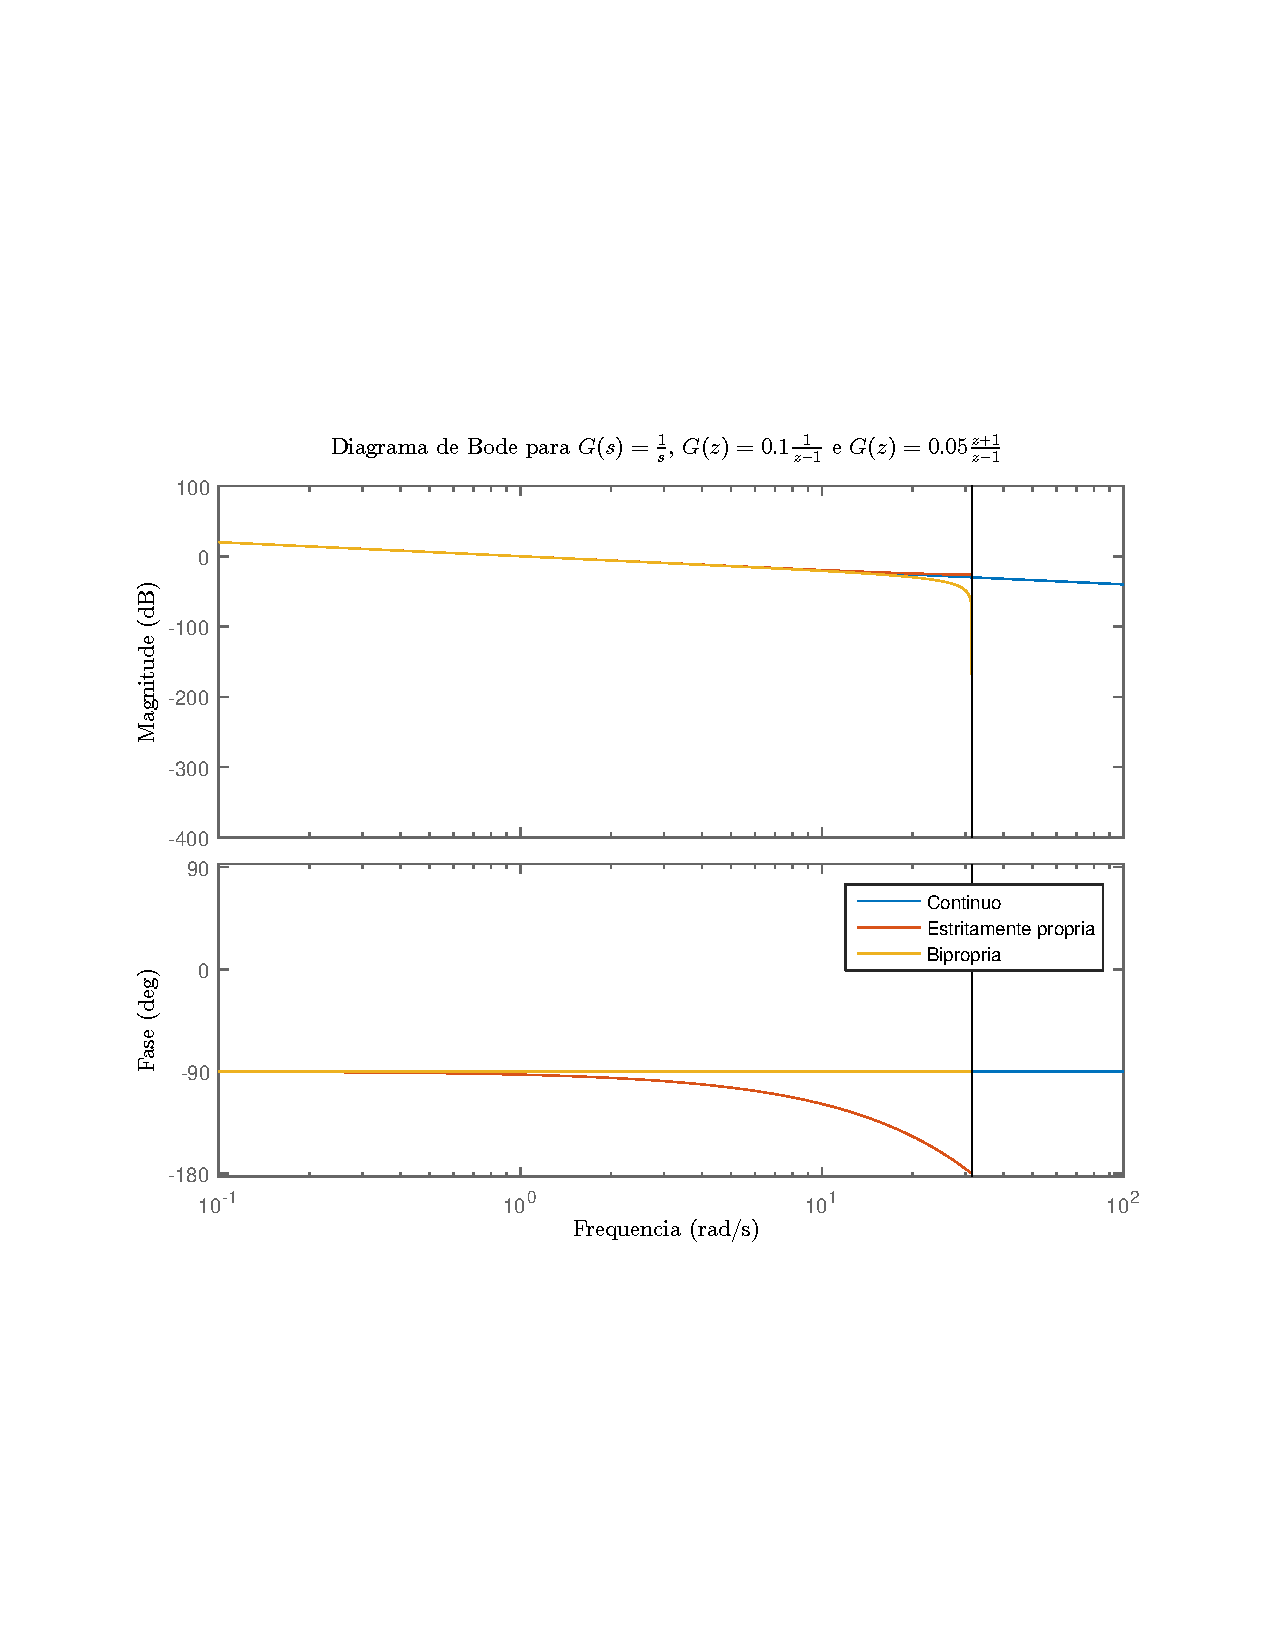
\includegraphics[width=\textwidth]{bodeex3.pdf}
        \caption{\label{fig:ex1ac} Diagrama de bode para as função de transferência contínua, discreta estritamente própria e biprópria} 
    \end{figure}

    \end{enumerate}
\newpage
\section*{Exercício 4}
\addcontentsline{toc}{section}{Exercício 4}

    A conversão sem aproximação do espaço contínuo para discreto com mantenedor de ordem zero (ZOH) satisfaz a seguinte equação:
    
        \begin{equation}
            G(z) \coloneqq (1-z^{-1}) \mathcal{Z}\left\{\mathcal{L}^{-1}\left\{\frac{G(s)}{s}\right\}\right\}
        \end{equation}
    
    Desta forma
    
        \begin{equation}
            \frac{G(s)}{s} = H(s) = \frac{K}{s(s+a)}
            \label{eq:ex41}
        \end{equation}
    
    Pelo método de expansão de frações parciais, a equação (\ref{eq:ex41}) apresenta a seguinte forma
    
        \begin{equation}
            H(s) = \frac{A}{s} + \frac{B}{(s+a)} 
        \end{equation}
    
    o qual 
    
        \begin{equation}
            A = H(s) s \bigg\rvert_{s=0} = \frac{K}{a} \mbox{ e } B = H(s) (s+a)\bigg\rvert_{s=-a} = -\frac{K}{a}
        \end{equation}
    
    Logo
    
        \begin{equation}
            H(s) = \frac{K}{a} \left( \frac{1}{s} - \frac{1}{s+a} \right)
        \end{equation}
    
    A função de transferência acima exceto ao fator de escala $j$ foi obtida no item (\ref{item:ex2b}). Desta forma
    
        \begin{equation}
            \mathcal{L}^{-1}\left\{\frac{G(s)}{s}\right\} = \frac{K}{a}\sigma(t)\left(1+e^{-at}\right)
            \label{eq:lapinv}
        \end{equation}
    
    Portanto, a função $\mathcal{Z}$ da função (\ref{eq:lapinv}) é dada por
    
        \begin{equation}
            G(z) = \frac{K}{a} \frac{(1 - e^{-aT_s}z^{-1})}{(1-z^{-1})(1 - e^{-aT_s}z^{-1})}
        \end{equation}
    
    Por fim, por meio da função de transefrência de uma malha fechada \footnote{A equação em malha fechada de um sistema em tempo discreto ou contínuo é dado pela equação $G_{MF}(z) = \frac{G(z)}{1+G(z)}$}, após certa manipulação algébrica é dada por:
    
        \begin{equation}
            G_{MF}(z) = K' \frac{z}{z+b}
        \end{equation}
        
    onde $K' = \frac{K}{a} (1-e^{-aT_s}) \mbox{ e } b = (1 + \frac{k}{a})\left[e^{-aT_s} - \frac{k}{a} \right] $.

\newpage
\section*{Exercício 5}
\label{ex:5}
\addcontentsline{toc}{section}{Exercício 5}
    

\newpage
\section*{Exercício 6}
\addcontentsline{toc}{section}{Exercício 6}

    Para os critérios de projeto fornecidos, o projeto de controle será feito em espaço $s$ e o respectivo pólo deve pertencer ao lugar das raízes em malha fechada. O tempo de subida é dado por:
    
        \begin{equation}
            t^{0\% - 100\%}_{r}(\omega_n, \zeta) = \frac{\pi - \theta(\zeta)}{\omega_d(\omega_n, \zeta)} \mbox{, com } \theta(\zeta) = \tan^{-1}\frac{\sqrt{1 - \zeta^2}}{\zeta} \mbox{ e } \omega_d(\omega_n, \zeta) = \omega_n \sqrt{1-\zeta^2}
            \label{eq:tempo_de_subida}
        \end{equation}
    
    De mesma forma, o sobressinal é dado por:
    
        \begin{equation}
            M(\zeta) = e^{-\pi \frac{\zeta}{\sqrt{1-\zeta^2}}}
            \label{eq:sobressinal}
        \end{equation}
    
    Como (\ref{eq:sobressinal}) é bijetora, $\exists g(M) = \zeta \mbox{, } g: M \longmapsto g(M) \mbox{, } M \circ g (M) = M$. De fato $g(M) = \sqrt{\frac{\log^2{M}}{\pi^2 - \log^2{M}}}$. Assim, $\zeta \approx 0.672$. De mesma forma, para $\zeta$ fixo, analogamente, $\exists h(t_r) = \zeta\mbox{, }h: t_r \longmapsto h(t_r)\mbox{, } t_r(\zeta) \circ h = t_r$. De fato, $g(t_r) = \frac{\pi - \theta}{\omega_d(\zeta, t_r)}$. Assim, para $\zeta = 0.672$, então $\omega_n = 4.46$.
    Por fim, $\forall s \in \mathbb{C}, \,\, s = \omega_n (\zeta + i \sqrt{1 - \zeta^2})$, logo a seguinte malha satisfaz os critérios estabelecidos em projeto
    
        \begin{equation}
        C(s) = K \frac{s + 0.7}{s + 2 \zeta \omega_n}
        \label{eq:Cs}
        \end{equation}
    
    O polinômio característico do sistema para \eqref{eq:Cs} em malha fechada é 
    
        \begin{equation}
        P(s) = s^2 + 2\zeta \omega_n + K \coloneqq 0
        \label{eq:polcarac}
        \end{equation}
    
    Ao considerar o projeto em tempo contínuo, o controlador acima "casa" o pólo da planta com o zero do controlador. Para o caso de casamento perfeito de pólo e zero, o novo lugar das raízes permite que o pólo estabelecido pertença a este. Ademais, para casamento perfeito de pólo e zero, por inspeção, o polinômio característico \eqref{eq:polcarac} fornece o valor $K$ para os pólos em projeto i.e., $K = \omega_n^2$. Assim, a função de transferência fornecida é:
    
        \begin{equation}
            C(s) = \omega_n^2 \frac{s + 0.7}{s + 2 \zeta \omega_n}
        \end{equation}
        
    Para projeto de controle por meio da aproximação do mantenedor de primeira ordem por transformação de Padé, utilizaremos a fórmula de Padé de primeira ordem seguinte:
    
    \begin{equation}
    e^{x} \approx \frac{1 + \frac{x}{2}}{1 - \frac{x}{2}}
    \label{eq:pade}
    \end{equation}
    
    Desta forma, por meio de \eqref{eq:pade}, a aproximação de padé exata pode ser aproximada por
    
    \begin{equation}
    G_{zoh}(s) = \frac{1 - e^{-T_s s}}{s T_s} \approx \frac{1}{\frac{T_s}{2} s + 1}
    \end{equation}
    
    A função de transferência em malha aberta do sistema é $G'(s) = C(s)*G_{zoh}(s)*G(s)$. De mesma forma ao projeto acima, o projeto de controlador em tempo discreto "casará" o pólo da planta com um zero do controlador. Para um controlador da forma \eqref{eq:controladorpade}, o pólo encontrado para projeto pertence a curva $1 + G'(s) \coloneqq 0$.   Com auxílio de software de manipulação numérica, encontramos $K$ e $p$ tal que o sistema satisfaça os critérios de  projeto. 
    
    A aproximação de Padé para o mantenedor de ordem zero no projeto do controlador aproxima o sinal em tempo discreto da ação contínua tanto para a saída, erro e ação de controle do sistema como representa as imagens \ref{fig:ex6saida}, \ref{fig:ex6erro} e \ref{fig:ex6controle}  respectivamente. Os diagramas de blocos utiliazdos para a simulação estão nas imagens \ref{fig:ex6continuo} e \ref{fig:ex6discreto}.
    
    \begin{equation}
    \label{eq:controladorpade}
        C(s) = K \frac{s + 0.7}{s + p}
    \end{equation}
    
    \begin{figure}[htp]
	\center
	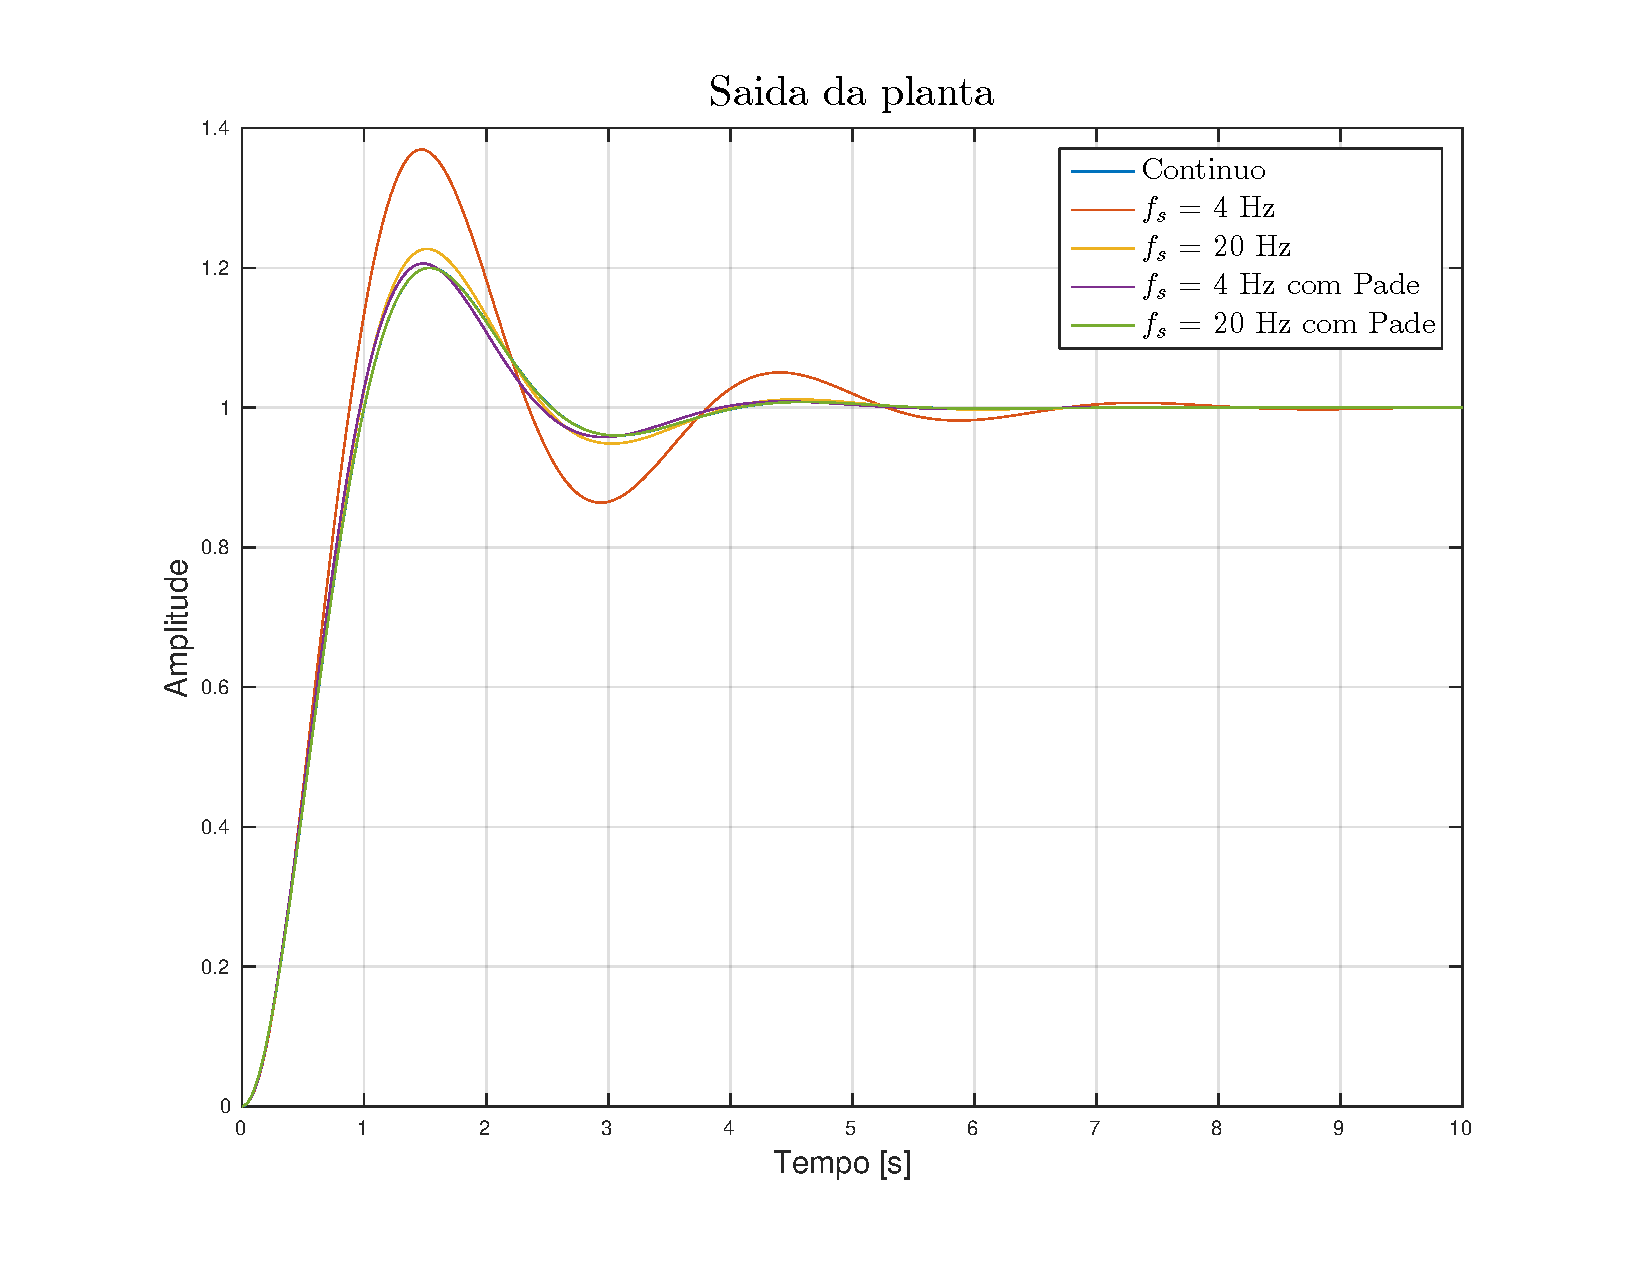
\includegraphics[width=0.8\textwidth]{images/saidazoh.pdf}
	\caption{Ação de controle para controle contínuo e discreto com $f_s = 4 Hz$ e $f_s = 20 Hz$. }
	\label{fig:ex6controle}
    \end{figure}
    
\newpage

    \begin{figure}[H]
	\center
	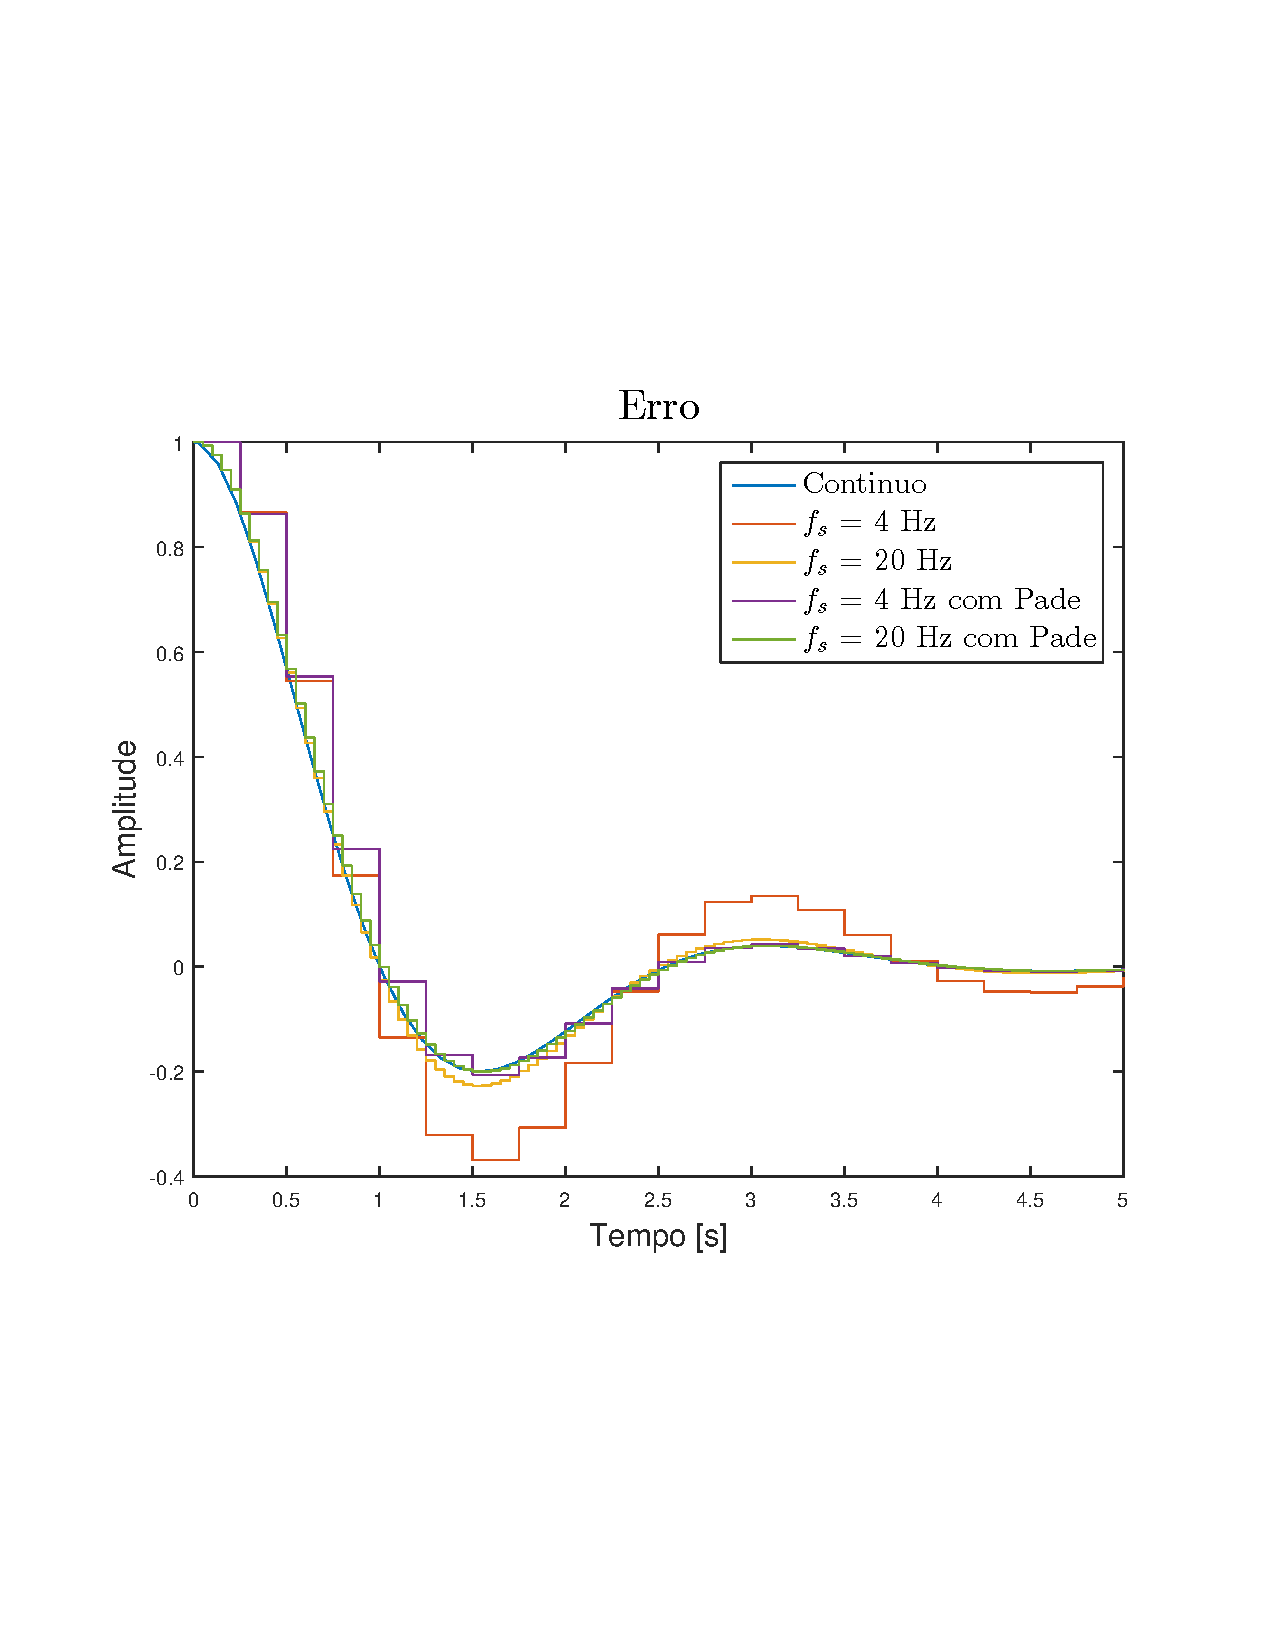
\includegraphics[width=0.8\textwidth]{images/controlezoh.pdf}
	\caption{Curva original e série amostrada}
	\label{fig:ex6saida}
    \end{figure}

    \begin{figure}[H]
	\center
	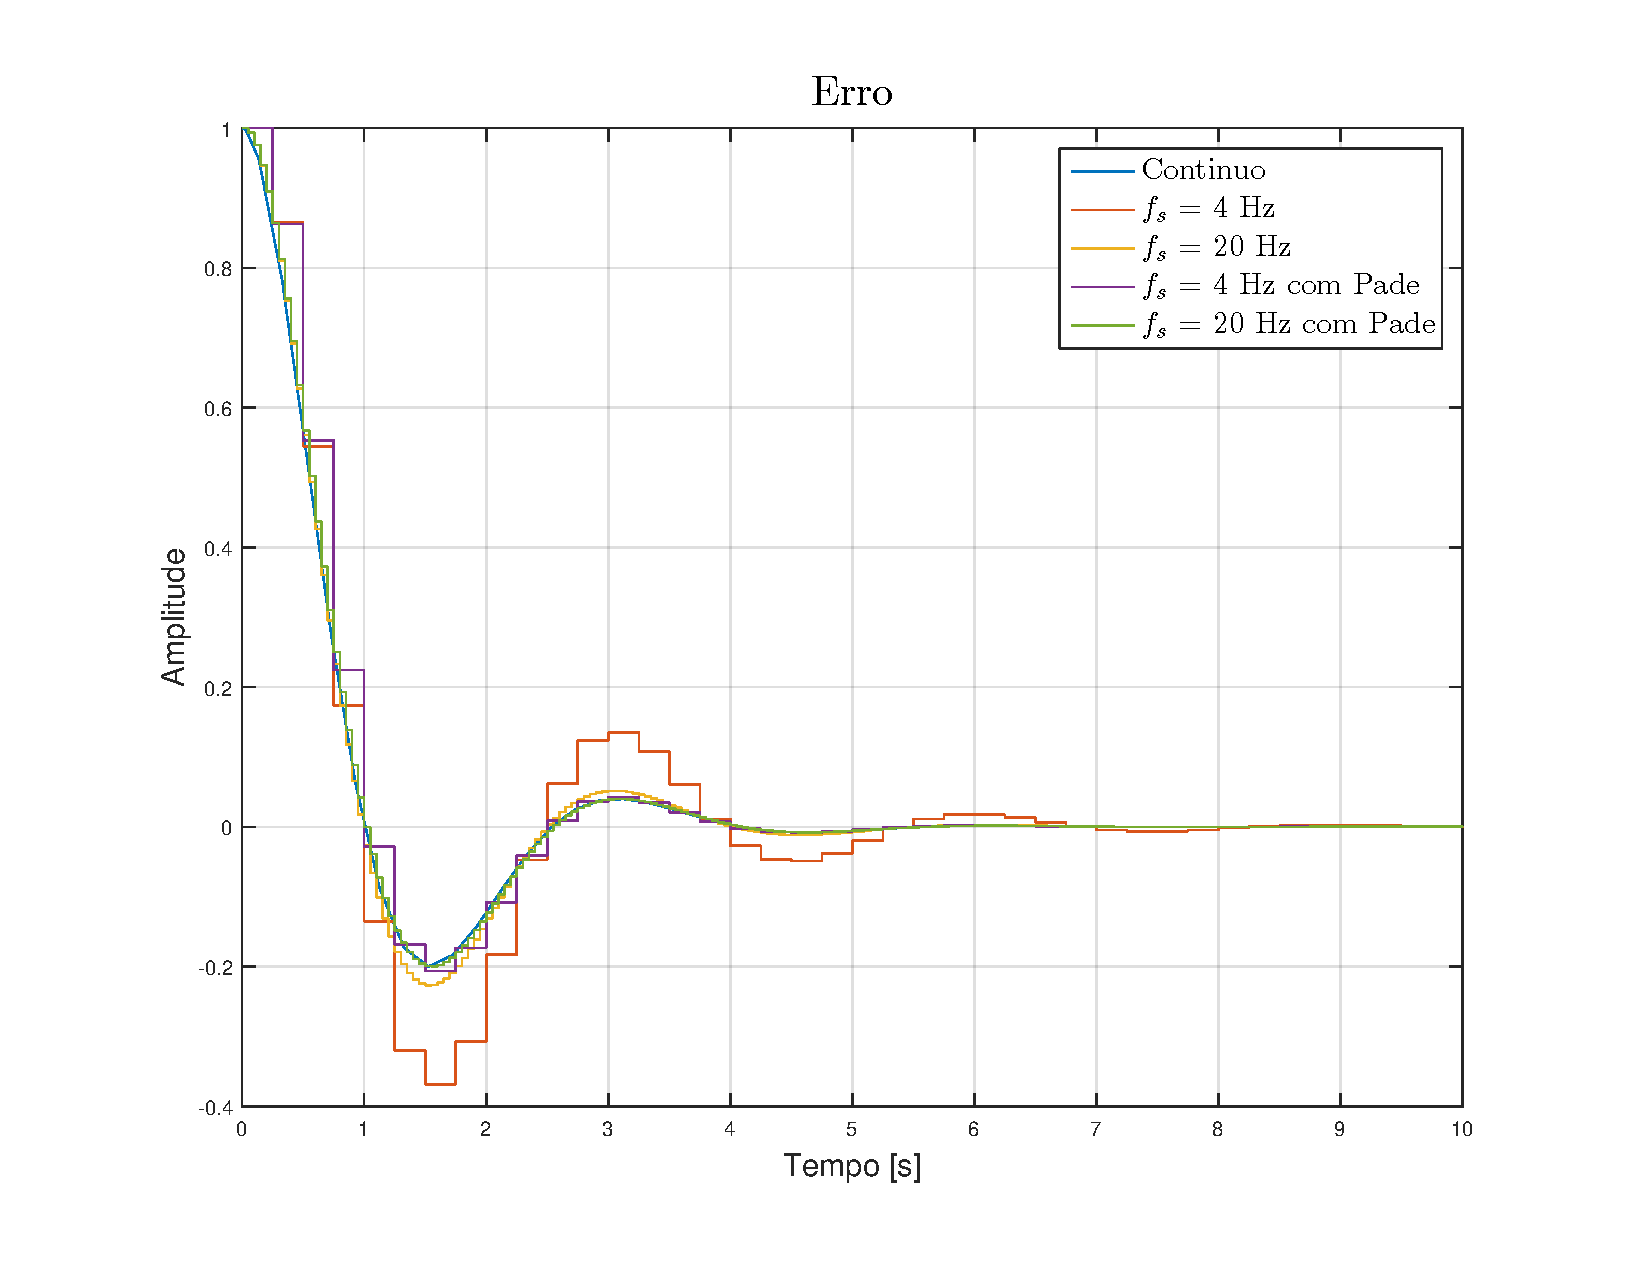
\includegraphics[width=0.8\textwidth]{images/errozoh.pdf}
	\caption{Curva original e série amostrada}
	\label{fig:ex6erro}
    \end{figure}
    
    \begin{figure}[H]
	\center
	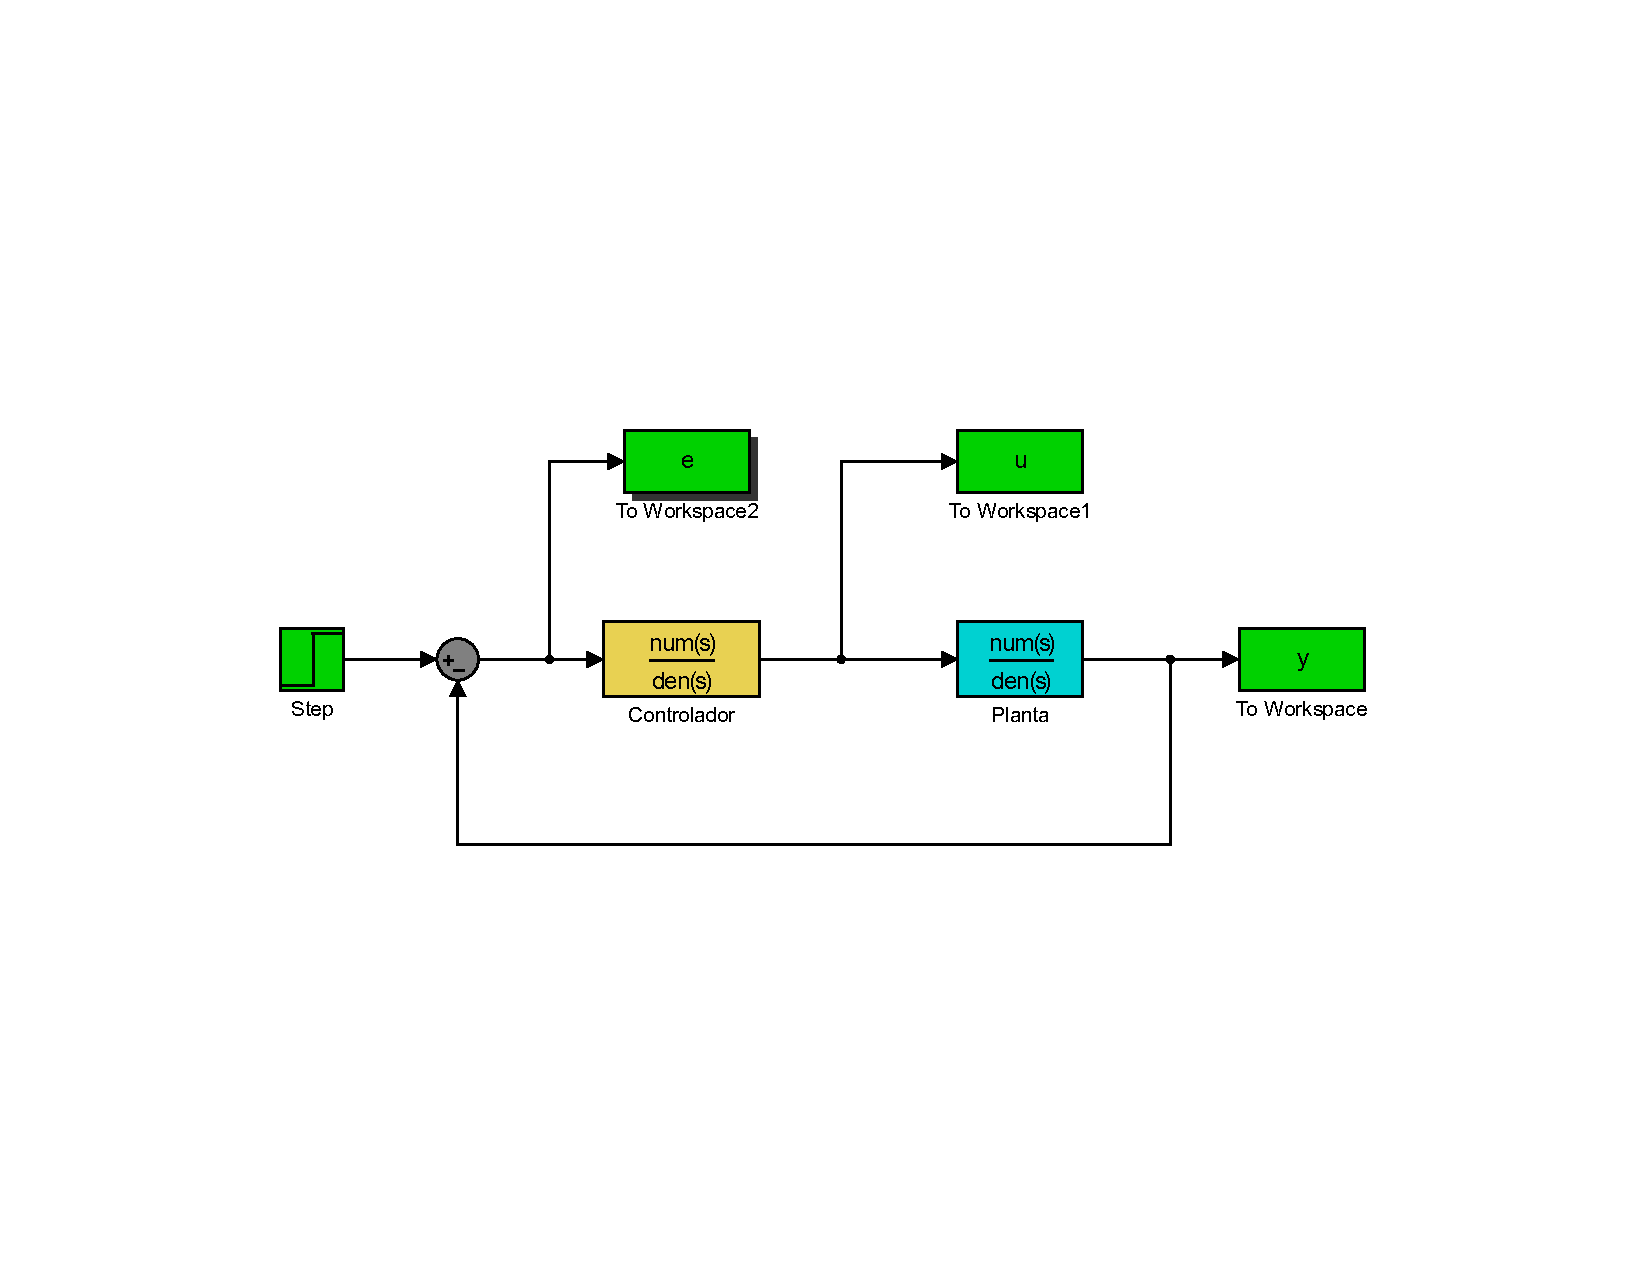
\includegraphics[width=0.8\textwidth]{images/ex6simcontinuo.pdf}
	\caption{Diagrama de blocos em malha fechada com controle contínuo}
	\label{fig:ex6continuo}
    \end{figure}

    \begin{figure}[H]
	\center
	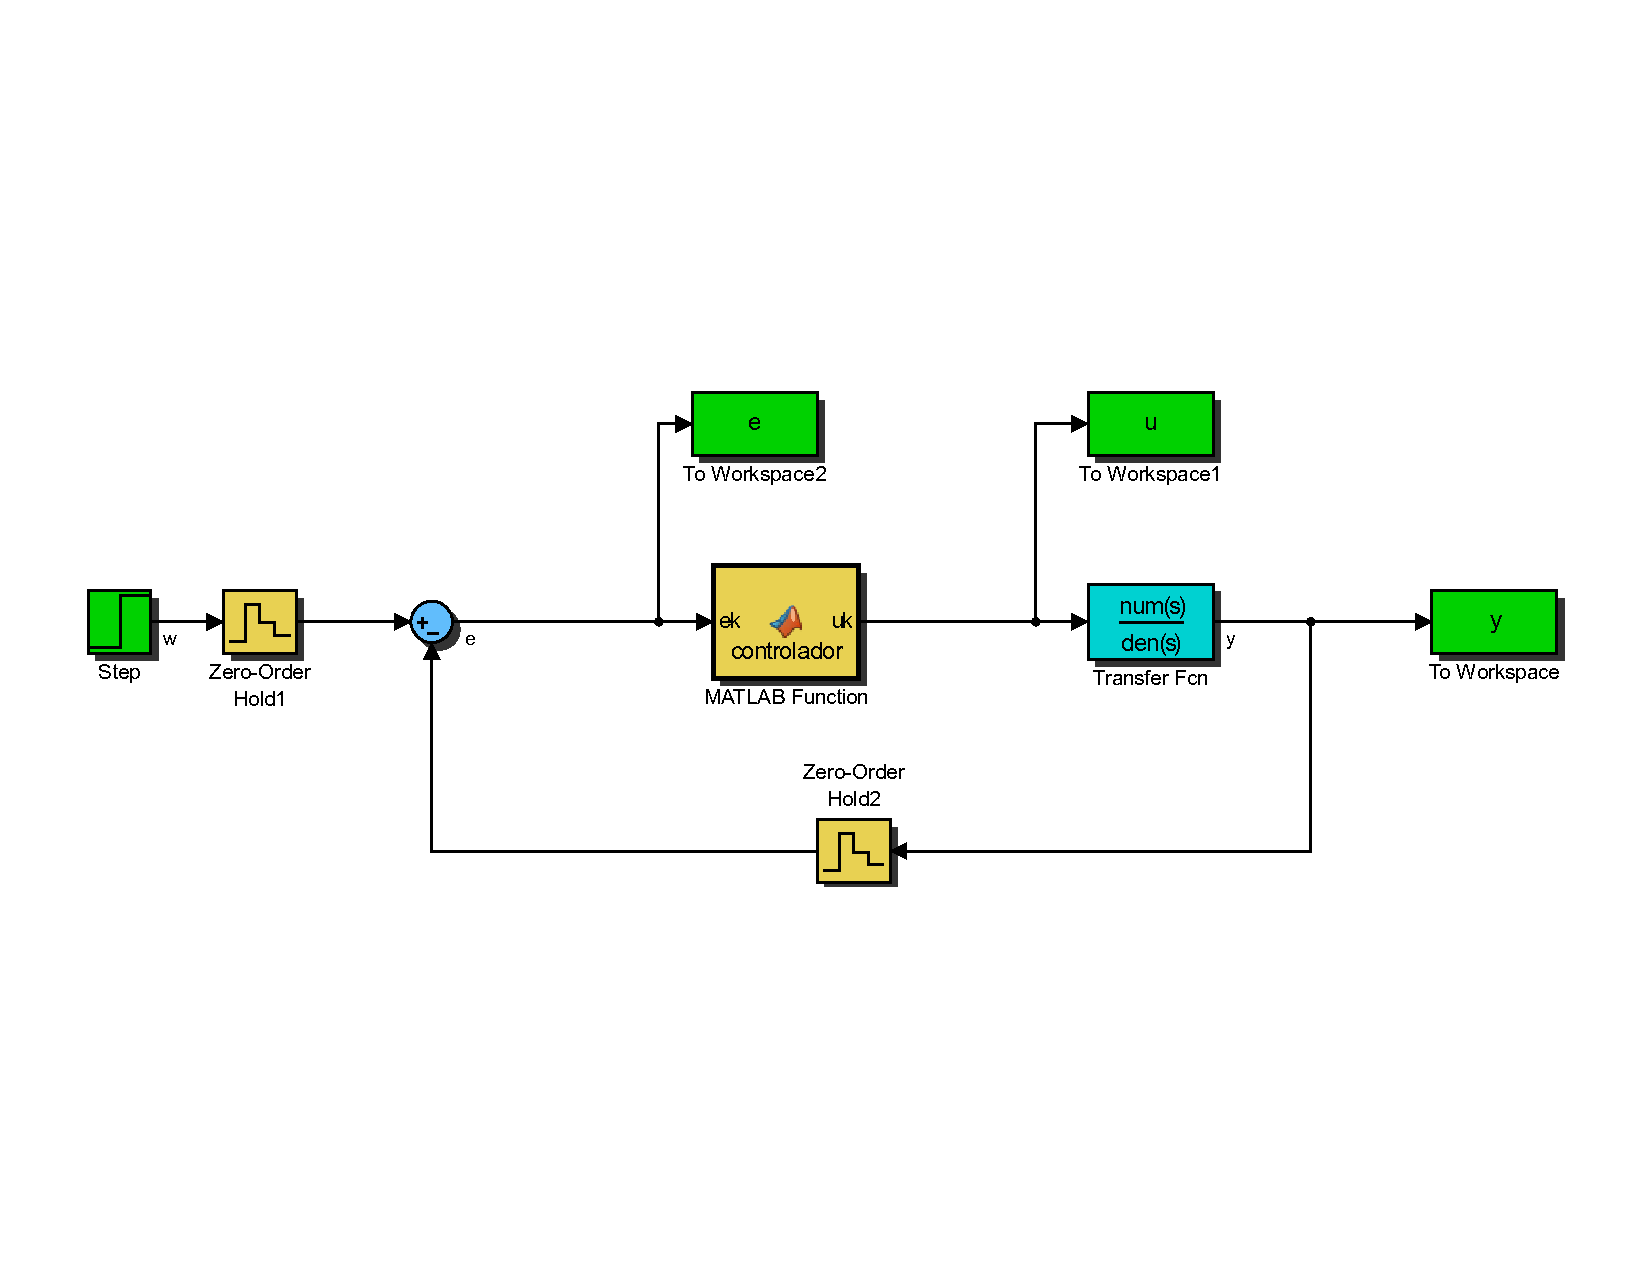
\includegraphics[width=0.8\textwidth]{images/ex6simdiscreto.pdf}
	\caption{Diagrama de blocos em malha fechada com controle discreto}
	\label{fig:ex6discreto}
    \end{figure}
\newpage
\section*{Exercício 7}
\label{ex:7}
\raggedbottom

Os dados utilizados na simulação tanto da planta quanto dos controladores estão nas tabelas \ref{tab:ex7planta} e \ref{tab:ex7controlador}. 

\begin{table}[H]
    \centering
    \begin{tabular}{|l|c|c|c|}
    \hline
    Descrição & Símbolo & Unidade & Valor \\ \hline
    Resistência do estator & R & $\Omega$ & 1 \\
    Indutância do estator & L & H & 0.01 \\
    Momento de inércia & J & kg $m^2$  & 1 \\
    Coeficiente de atrito viscoso & b & $Ns$ & 0.01 \\
    Fator transformação eletromagnética & K & NmA & 1 \\\hline
    \end{tabular}
    \caption{Parâmetros da planta}
    \label{tab:ex7planta}
\end{table}

\begin{table}[H]
    \centering
    \begin{tabular}{|l|c|c|c|}
    \hline
    Descrição & Símbolo & Unidade & Valor \\ \hline
    Ganho proporcional & $K_p$ & $N \frac{rad}{s}$ & 18 \\
    Constante de tempo integrativo & $T_i$ & s & 0.42 \\
    Constante de tempo derivativo & $T_d$ & s  & 0.05 \\
    Período de amostragem & $T_s$ & s & 0.01 \\\hline
    \end{tabular}
    \caption{Parâmetros dos controladores}
    \label{tab:ex7controlador}
\end{table}

A utilização da estratégia anti-windup juntamente ao controlador PID reduz o tempo que o controlador necessita para sair da área de saturação. O intervalo de tempo que o controlador permanece em saturação na imagem \ref{fig:PIDantiwindup} não é suficiente para afirmar categoricamente a respeito da conclusão acima com os dados fornecidos no enunciado. Entretanto, por meio do aumento do \emph{set-point}, o aluno observou o fato.

Ao compararmos controladores PID, ambos com estratégia anti-windup, sem e com filtro passa-baixas na ação derivativa, é possível observarmos uma diminuição na sensibilidade ao ruido de leitura, o que faz com que o sinal convirja de forma mais suave que o sinal sem o filtro.

Por fim, como análise final, o aluno escolheu duas estratégias apresentadas na apostila da disciplina. A primeira não acresce a ação integral durante o período de saturação e a segunda, além disto, mitiga o sinal de controle por meio de um fator proporcional à diferença de ação de controle antes e depois da saturação. 

\begin{figure}[!h]
    \center
    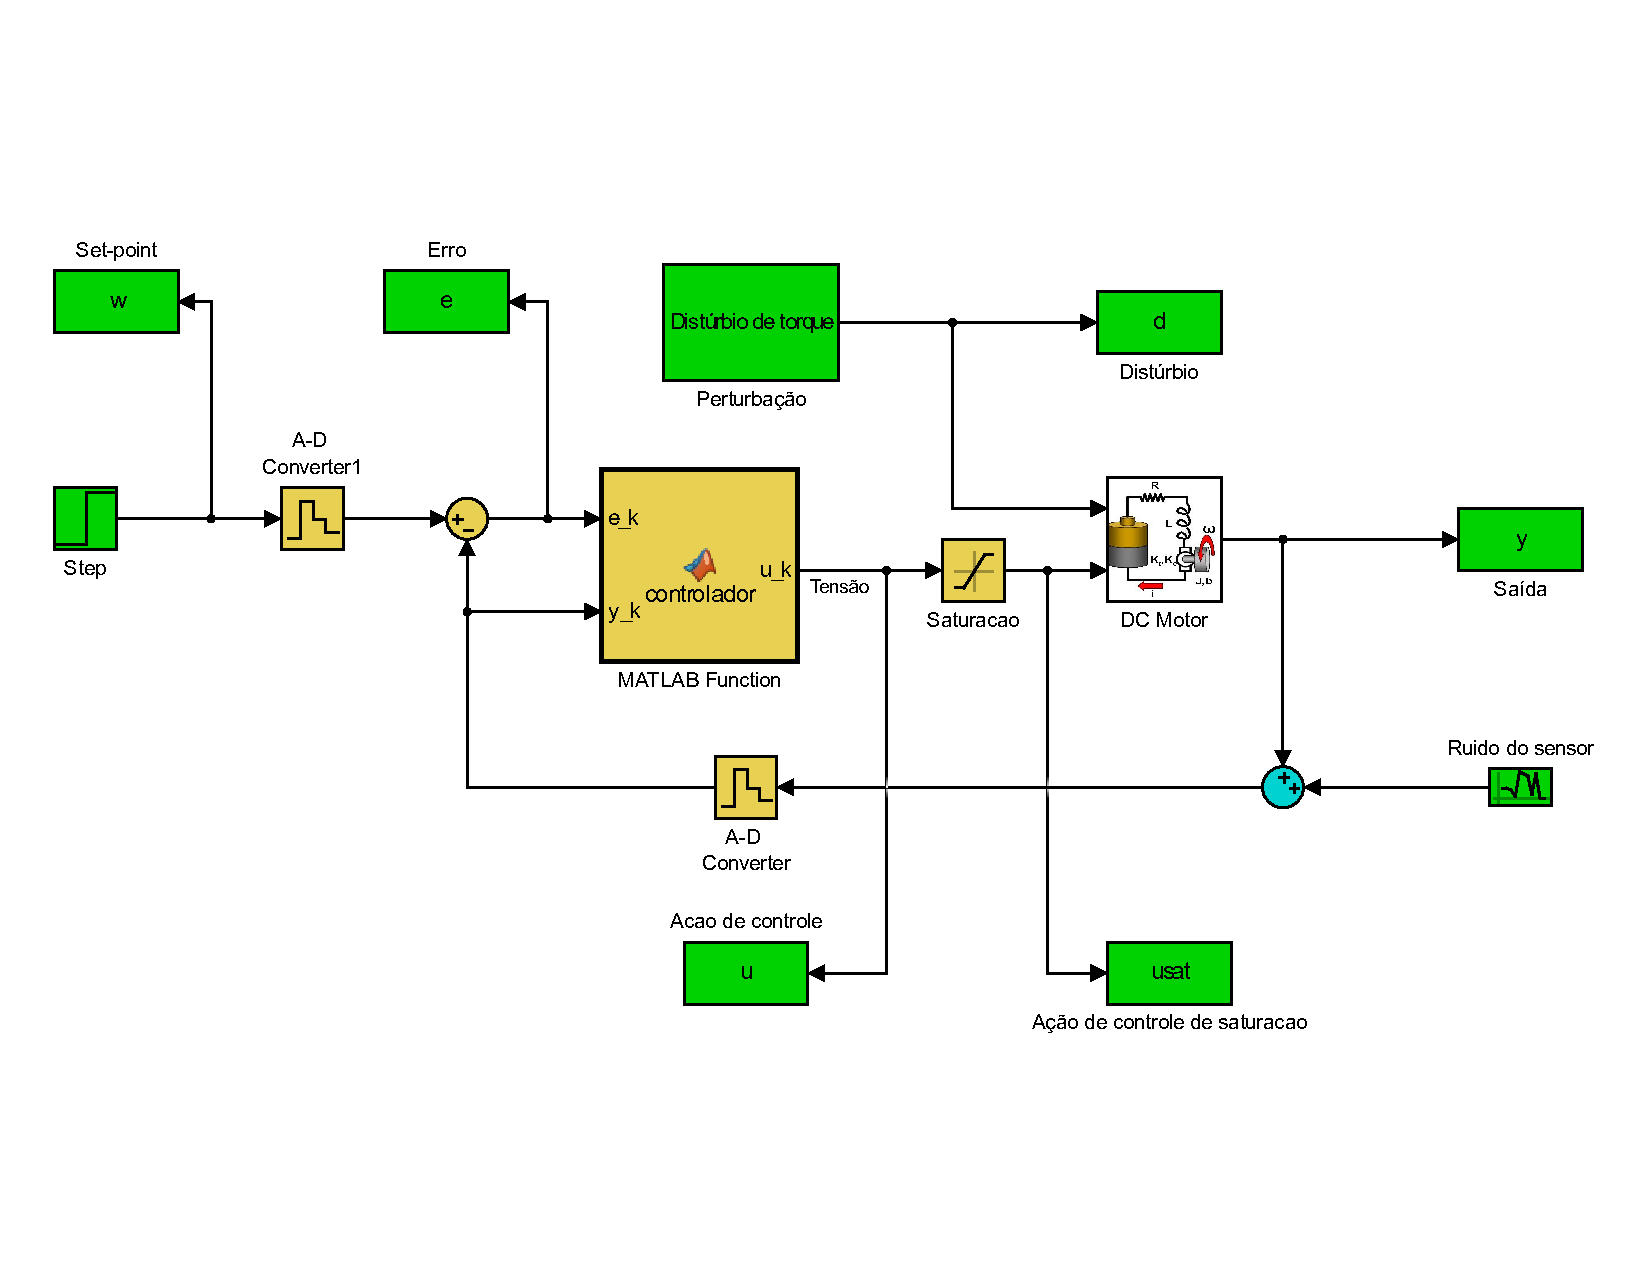
\includegraphics[width=0.8\textwidth, trim=4cm 3.5cm 1cm 2cm]{dcIntrocomplete.pdf}
    \caption{Principais sinais de controle do diagrama} 
    \label{fig:dcIntrocomplete}
\end{figure}

\begin{figure}[H]
    \center
    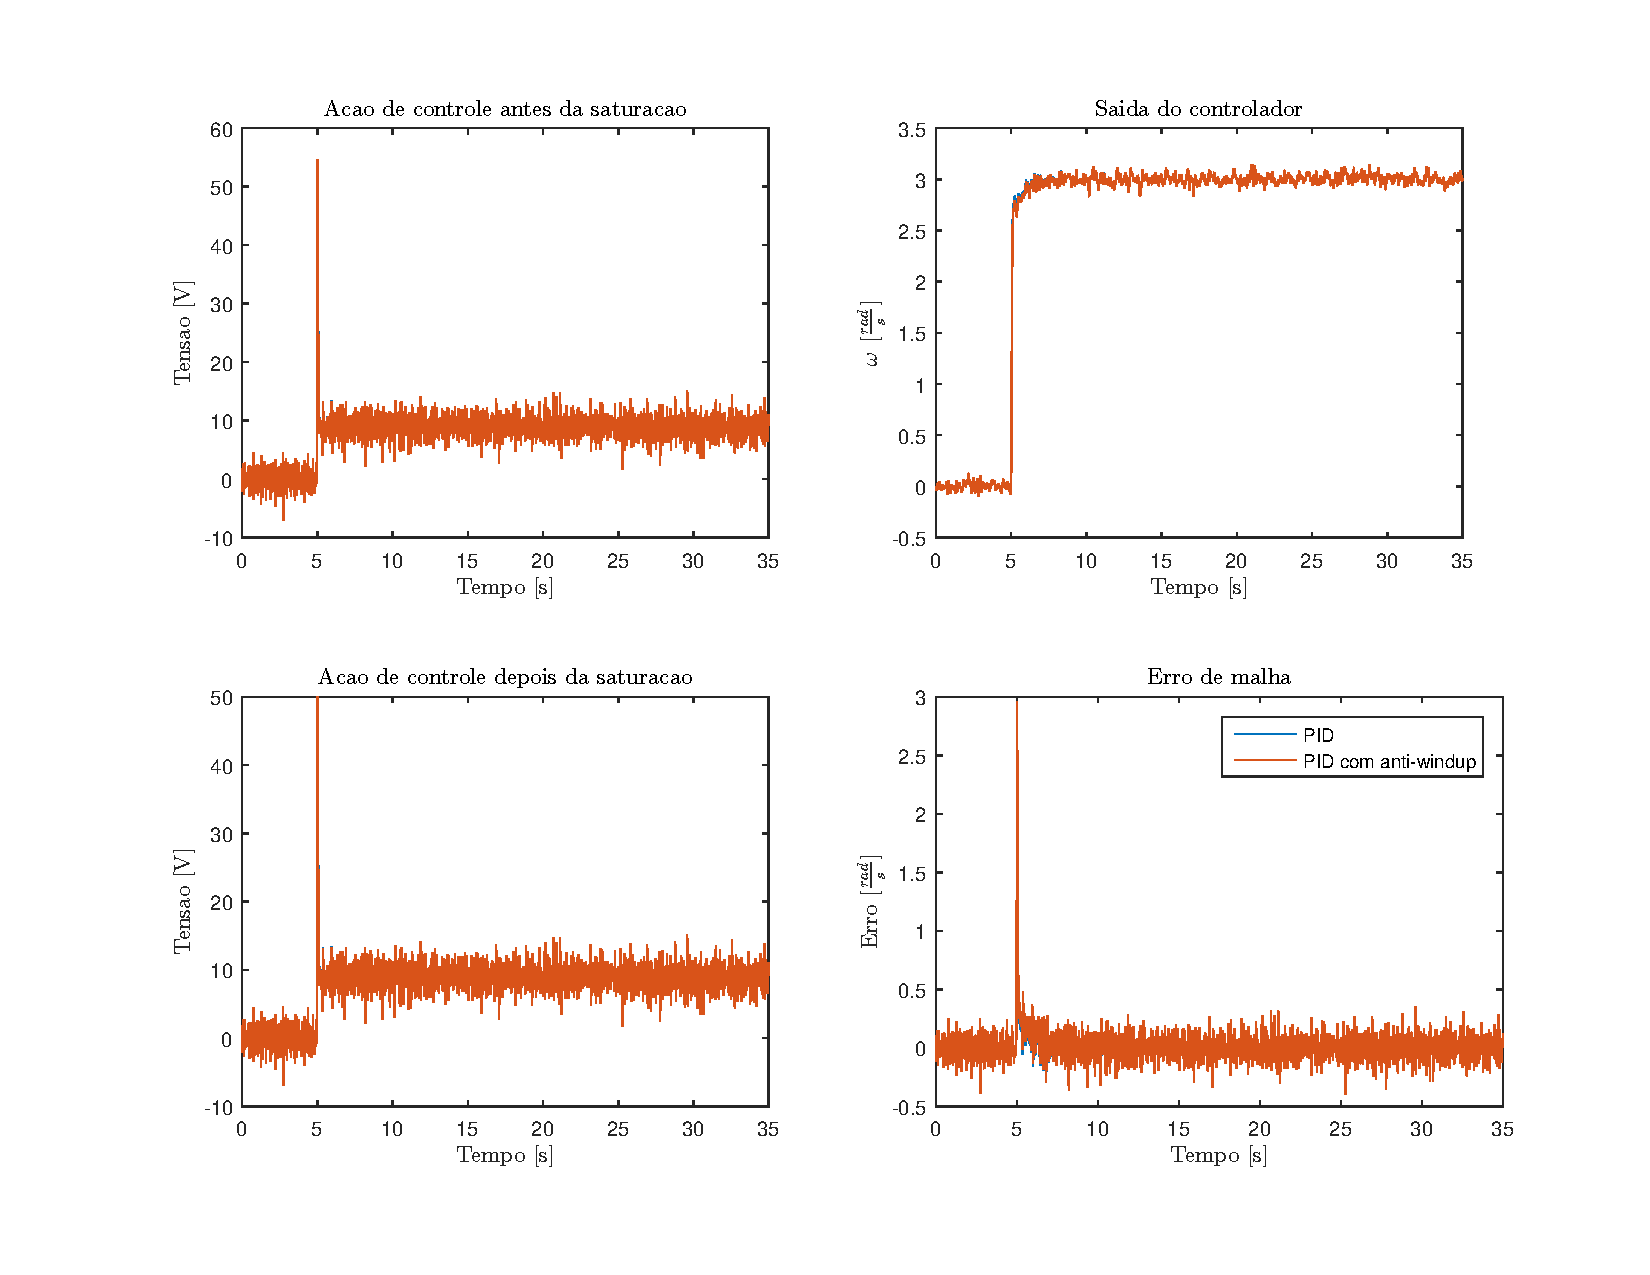
\includegraphics[width=0.85\textwidth, trim=3.5cm 2cm 2cm 1cm]{ex7PID_PIDantiwindup.pdf}
    \caption{Diagrama de blocos utilizado para exercício 7}
    \label{fig:PIDantiwindup}
\end{figure}

\begin{figure}[H]
    \center
    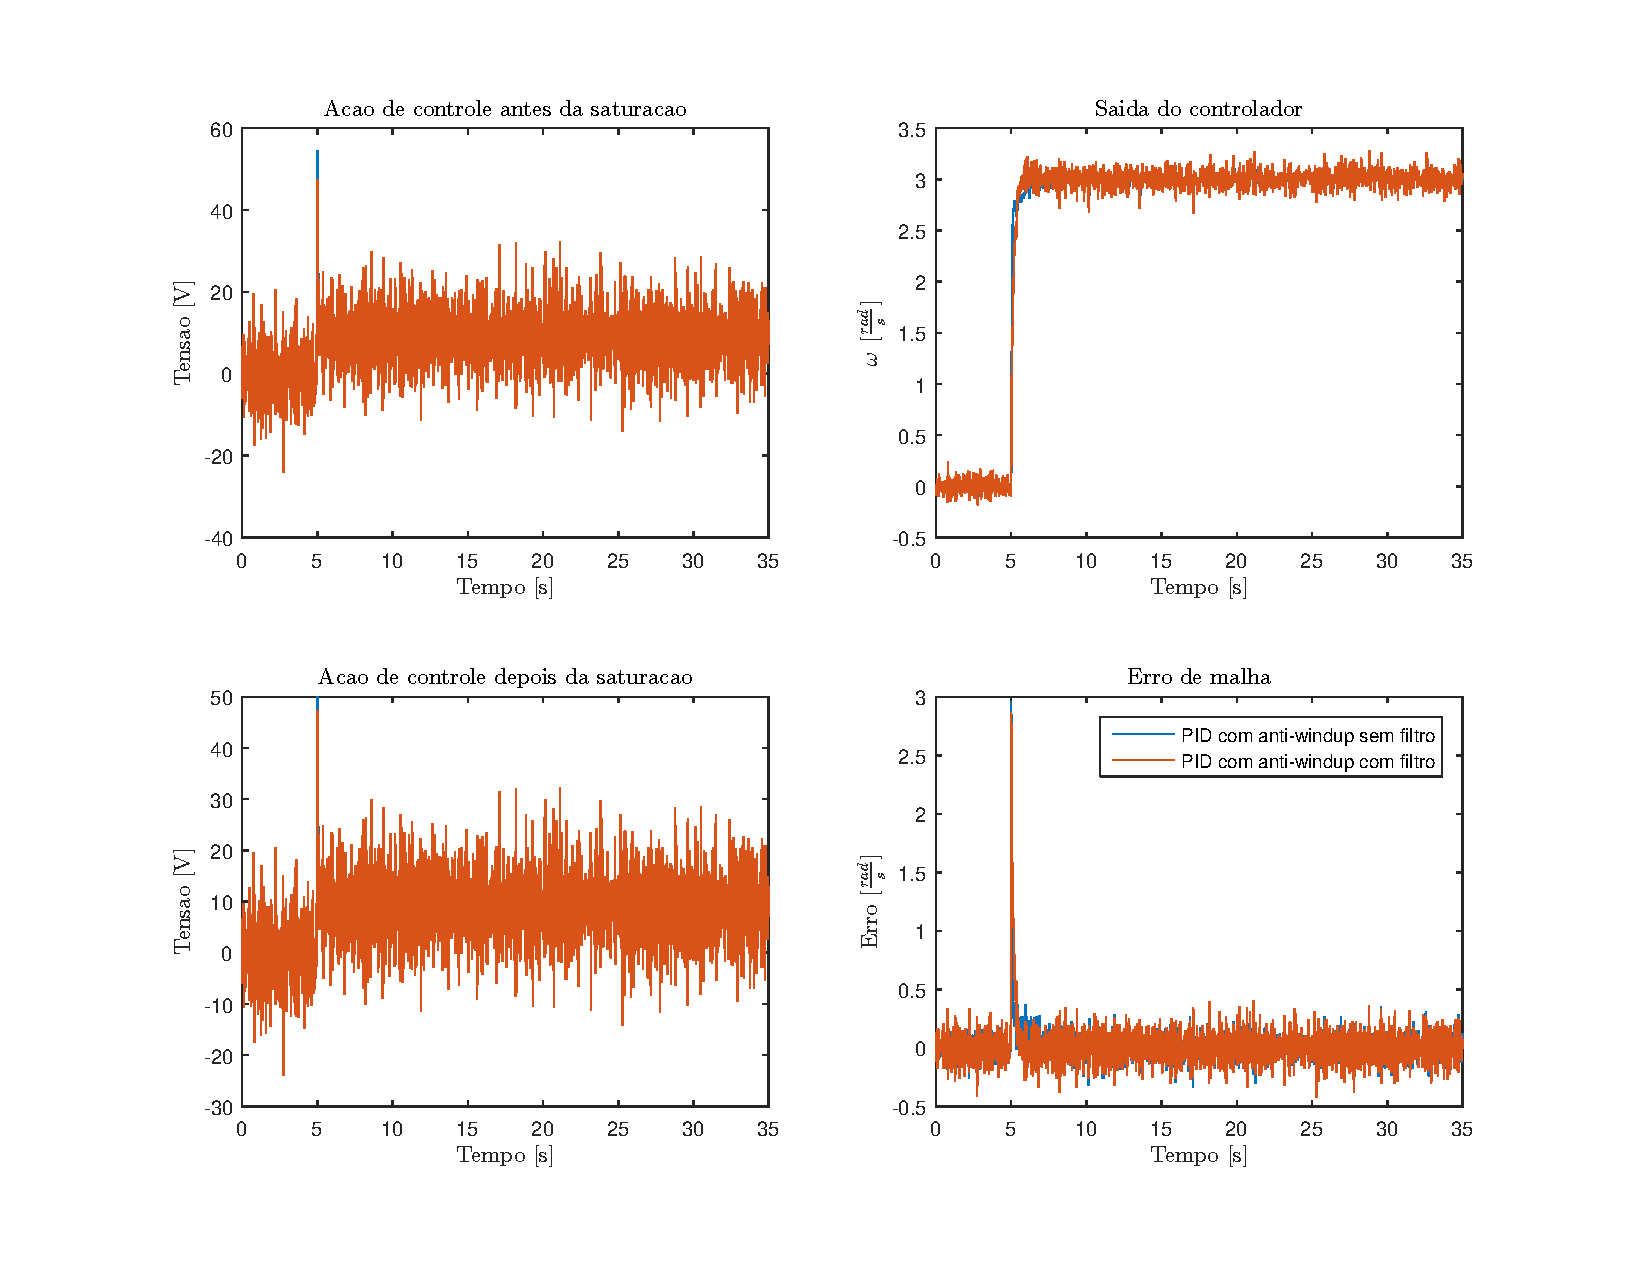
\includegraphics[width=0.8\textwidth, trim=3.5cm 2.5cm 2cm 2cm]{ex7PID_antiwindup_filtro.pdf}
    \caption{Diagrama de blocos utilizado para exercício 7}
    \label{fig:PIDfiltro}
\end{figure}

\begin{figure}[H]
    \center
    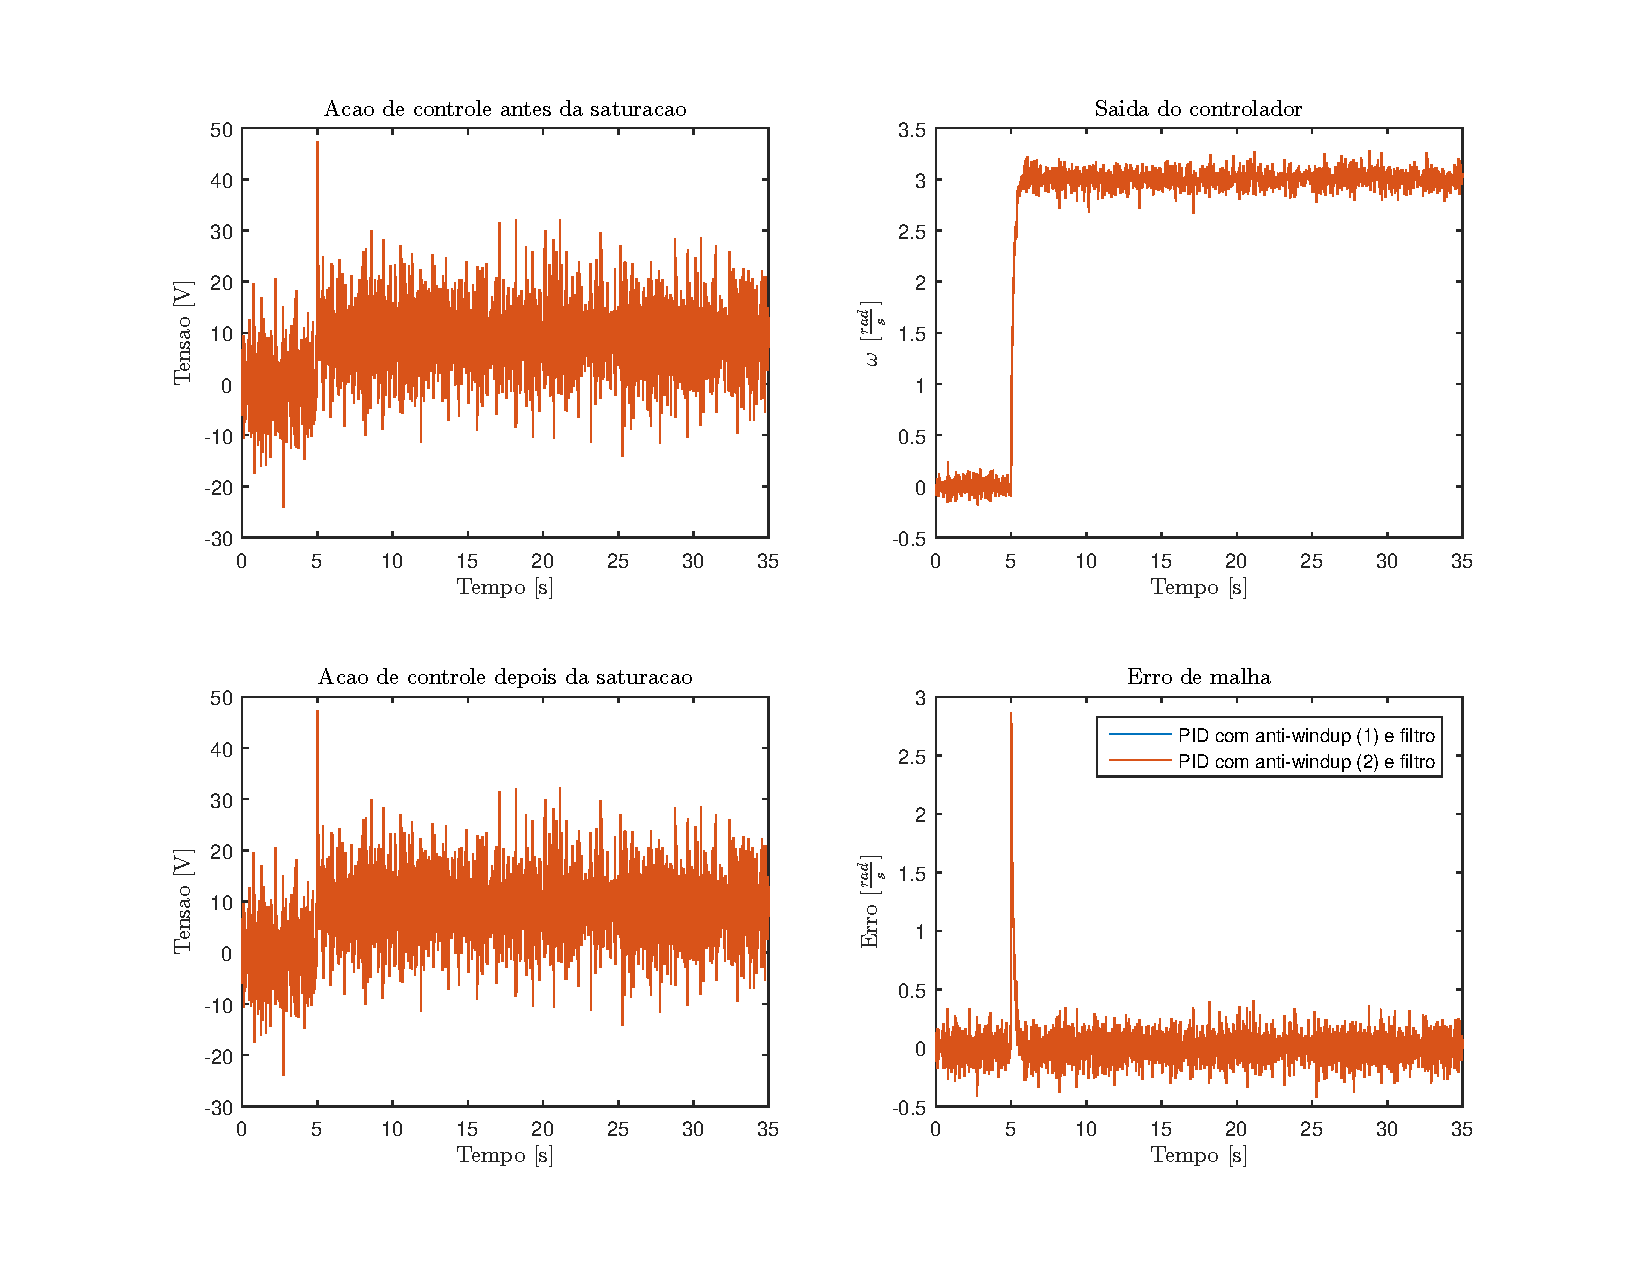
\includegraphics[width=0.8\textwidth, trim=3.5cm 2.5cm 2cm 2cm]{PID_antiwidup12_filtro.pdf}
    \caption{Diagrama de blocos utilizado para exercício 7}
    \label{fig:PIDantiwindup12}
\end{figure}

\newpage
\section*{Exercício 8}
\label{ex:8}

\addcontentsline{toc}{section}{Exercício 8}

    A transformação para trás tem parâmetros $c^T = [1, -1]$ e $d^T = [T_s, 0]$ e a transformação para frente $c^T = [1, -1]$ e $d^T = [0, T_s]$. A implementação em MatLab encontra-se em anexo.
\newpage
%---------------------------------------------------------------------------

%--------------------------------- Anexos ----------------------------------
\section*{Scripts}
    \subsection*{ex6.m}
    \label{subsec:ex6}
    \lstinputlisting[language=Matlab, caption=Script utilizado para resolução do exercício 6]{code/ex6/ex6.m}

    \subsection*{sim\_ex6.m}
    \label{subsec:simex6}
    \lstinputlisting[language=Matlab, caption=Script utilizado para simulação dos modelos em Simulink do exercício 6]{code/ex6/sim_ex6.m}

    \subsection*{plot\_ex6.m}
    \label{subsec:plotex6}
    \lstinputlisting[language=Matlab, caption=Script utilizado para visualização das imagens do exercício 6]{code/ex6/plot_ex6.m}
    
    \subsection*{mfunctioncontent.m}
    \label{subsec:mfunctioncontent}
    \lstinputlisting[language=Matlab, caption=Conteúdo da função MatLab no diagrama de blocos com controle discreto do exercício 6]{code/ex6/mfunctioncontent6.m}

    \subsection*{syms2tfz.m}
    \label{subsec:syms2tfz}
    \lstinputlisting[language=Matlab, caption=Conversão de simbólico fracionário em função de transferência discreta]{code/syms2tfz.m}
    
    \subsection*{s2z.m}
    \label{subsec:s2z}
    \lstinputlisting[language=Matlab, caption=Conversão de função de transferência por transformação $T(z)$]{code/s2z.m}
    
    \subsection*{backward.m}
    \label{subsec:backward}
    \lstinputlisting[language=Matlab, caption=Transformação de conversão para trás]{code/backward.m}
    
    \subsection*{forward.m}
    \label{subsec:forward}
    \lstinputlisting[language=Matlab, caption=Transformação de conversão para frente]{code/forward.m}
    
    \subsection*{tustin\_prop.m}
    \label{subsec:tustin}
    \lstinputlisting[language=Matlab, caption=Transformação de conversão tustin própria]{code/tustin_prop.m}
%---------------------------------------------------------------------------

\phantomsection
\addcontentsline{toc}{section}{referências}
\printbibliography 

\end{document}
